\documentclass[sigconf,nonacm]{acmart}
\usepackage{booktabs}
\usepackage{url}
\usepackage{amsmath}
\settopmatter{printacmref=false,printccs=false,printfolios=true,authorsperrow=3}
\setcopyright{none}
\renewcommand\footnotetextcopyrightpermission[1]{}
\pagestyle{plain}
\setlength{\emergencystretch}{1em}
\setlength{\dbltextfloatsep}{6pt plus 2pt minus 2pt}
\setlength{\textfloatsep}{8pt plus 2pt minus 2pt}

\title{PRISM: Evaluating Privacy-Constrained Feature Tiers for Customer Churn Classification}
\titlenote{Code and results: \url{https://github.com/ParsanaDev/PRISM-churn-privacy/tree/milestone4-evaluation}}
\author{Abhishek Majumdar}
\affiliation{\institution{University of Victoria}\city{Victoria}\country{Canada}}
\author{Dev Parsana}
\affiliation{\institution{University of Victoria}\city{Victoria}\country{Canada}}
\author{Ravi Vashi}
\affiliation{\institution{University of Victoria}\city{Victoria}\country{Canada}}
\renewcommand{\shortauthors}{Majumdar et al.}

\begin{document}
\begin{abstract}
PRISM asks how much churn-prediction quality is lost when a model may only use less personal customer data. On the IBM Telco data we define three nested feature tiers (administrative terms; + billing; + demographics and services) and evaluate a $k$-NN baseline and a logistic regression (LR) model under one shared protocol: a stratified 80/20 hold-out split, a stratified 5-fold CV, and selection by mean F-measure. Adding billing data increases the test F-measure by 0.03 in LR and 0.09 in $k$-NN; adding demographics and services adds 0.04, 0.06 more respectively. Neither model wins on every metric: LR is ahead on PR-AUC in every tier, but $k$-NN has the higher ROC-AUC and F-measure in Tier~2. Also LR is far more sensitive to its hyperparameters as compared to $k$-NN.
\end{abstract}
\keywords{customer churn, data minimization, privacy tiers, $k$-NN, logistic regression}
\maketitle

\section{Introduction}
Churn models are usually trained on everything a provider knows about its customers~\cite{mozer,neslin}, while data-minimization work asks how much input a model actually needs~\cite{goldsteen}. PRISM fixes the learning protocol and varies only the information a model may see. Unlike feature selection by predictive power~\cite{omari}, each tier is fixed \emph{before} training. This report will evaluate the method defined in milestone 3.

\section{Research Questions}
\textbf{RQ1 (Inference performance):} \emph{How does churn classification change as a model gets access to more personal tiers, and does LR outperform the $k$-NN baseline in each tier?} This measures the cost of data minimization and whether a parametric model uses limited features better than a non-parametric one. We compare both models with their best settings on the hold-out test set (Table~\ref{tab:rq1}).

\textbf{RQ2 (Hyperparameter sensitivity):} \emph{How sensitive is each model to its hyperparameters in each tier?} A model that needs careful tuning is harder to deploy reliably. We report the range of the mean 5-fold CV F-measures across all settings instead of the entire $k$ sweep and the LR grid (Table~\ref{tab:rq2}).

\section{Dataset}
We use the public IBM Telco Customer Churn data~\cite{ibmtelco}: 7,043 customers and 33 columns, with binary label \emph{Churn Value} (1,869 churners, 26.5\%). It is a widely used churn benchmark, it is labelled, and its columns range from administrative to personal, which is exactly what our tiers need. Tier~1 has 4 attributes (tenure, contract, payment method, paperless billing), Tier~2 adds monthly and total charges (total 6 labels), and Tier~3 adds demographics and subscribed services (all 19 labels). Identifiers, location and outcome-derived fields (Churn Score, CLTV, Churn Reason) are never used. The only missing values are 11 blank Total Charges, all for zero-tenure customers, which we set to 0; no duplicates were found. The same cleaning process applies to every model and tier.

\section{Baselines}
\textbf{$k$-NN (baseline)} predicts churn by majority vote of the $k$ nearest training customers under Euclidean distance. It is non-parametric, assumes no boundary shape and has one hyperparameter, so it is a transparent reference. We sweep $k\in\{1,\dots,20\}$ (scikit-learn).
\textbf{Logistic regression} scores a customer with $\sigma(\mathbf{w}^\top\mathbf{x}+b)$ and predicts churn at $\ge0.5$. Following the course notebook it is trained to minimise the absolute error $|y-\hat y|$ by mini-batch gradient descent written in NumPy. It is parametric and interpretable, a conceptually different competitor to $k$-NN. We apply learning rate $\eta\in\{0.01,0.1,0.5\}$, epochs $T\in\{50,200\}$ and batch size $|B|\in\{32,128,512\}$ (18 settings) while running LR. Both models receive the same inputs: numeric attributes z-scored and categorical attributes one-hot encoded, fitted on training rows only.

\section{Evaluation Strategy and Metrics}
The data is split once, stratified on churn, into a development set (5,634) and a final test set (1,409, including 374 churners). The development set is divided into five stratified folds, and every model, tier and setting uses the same folds (seed 2026). For each setting we average the fold F-measures, pick the best, refit on the whole development set and score the test set \emph{once}; the test set never influences a choice. Churn is defined as the positive class and since classes are imbalanced (26.5\%), we do not report accuracy, instead we use F-measure for selection (it balances missed churners and false alarms), precision and recall to explain it, ROC-AUC for ranking quality across thresholds, and average precision (reported as PR-AUC) for minority-class ranking.

\section{Results and Discussion}
\begin{table}[t]
\caption{RQ1: hold-out test results (1,409 customers, 374 churners) with each model's CV-selected setting. Best per tier in bold.}\label{tab:rq1}
\small\setlength{\tabcolsep}{2.6pt}
\begin{tabular}{@{}llcccccc@{}}
\toprule
Tier & Model & Setting & P & R & F & ROC & PR\\
\midrule
1 & $k$-NN & $k{=}15$ & 0.551 & 0.436 & 0.487 & 0.781 & 0.517\\
  & LR & 0.5/200/32 & \textbf{0.589} & \textbf{0.495} & \textbf{0.538} & \textbf{0.782} & \textbf{0.568}\\
2 & $k$-NN & $k{=}13$ & \textbf{0.620} & \textbf{0.545} & \textbf{0.580} & \textbf{0.815} & 0.591\\
  & LR & 0.5/200/32 & 0.608 & 0.527 & 0.564 & 0.807 & \textbf{0.629}\\
3 & $k$-NN & $k{=}19$ & 0.623 & \textbf{0.623} & \textbf{0.623} & 0.838 & 0.630\\
  & LR & 0.5/50/32 & \textbf{0.659} & 0.588 & 0.621 & \textbf{0.842} & \textbf{0.661}\\
\bottomrule
\end{tabular}
\\[1pt]{\footnotesize LR setting: $\eta$/epochs/batch size.}
\end{table}

\begin{figure*}[t]
\centering
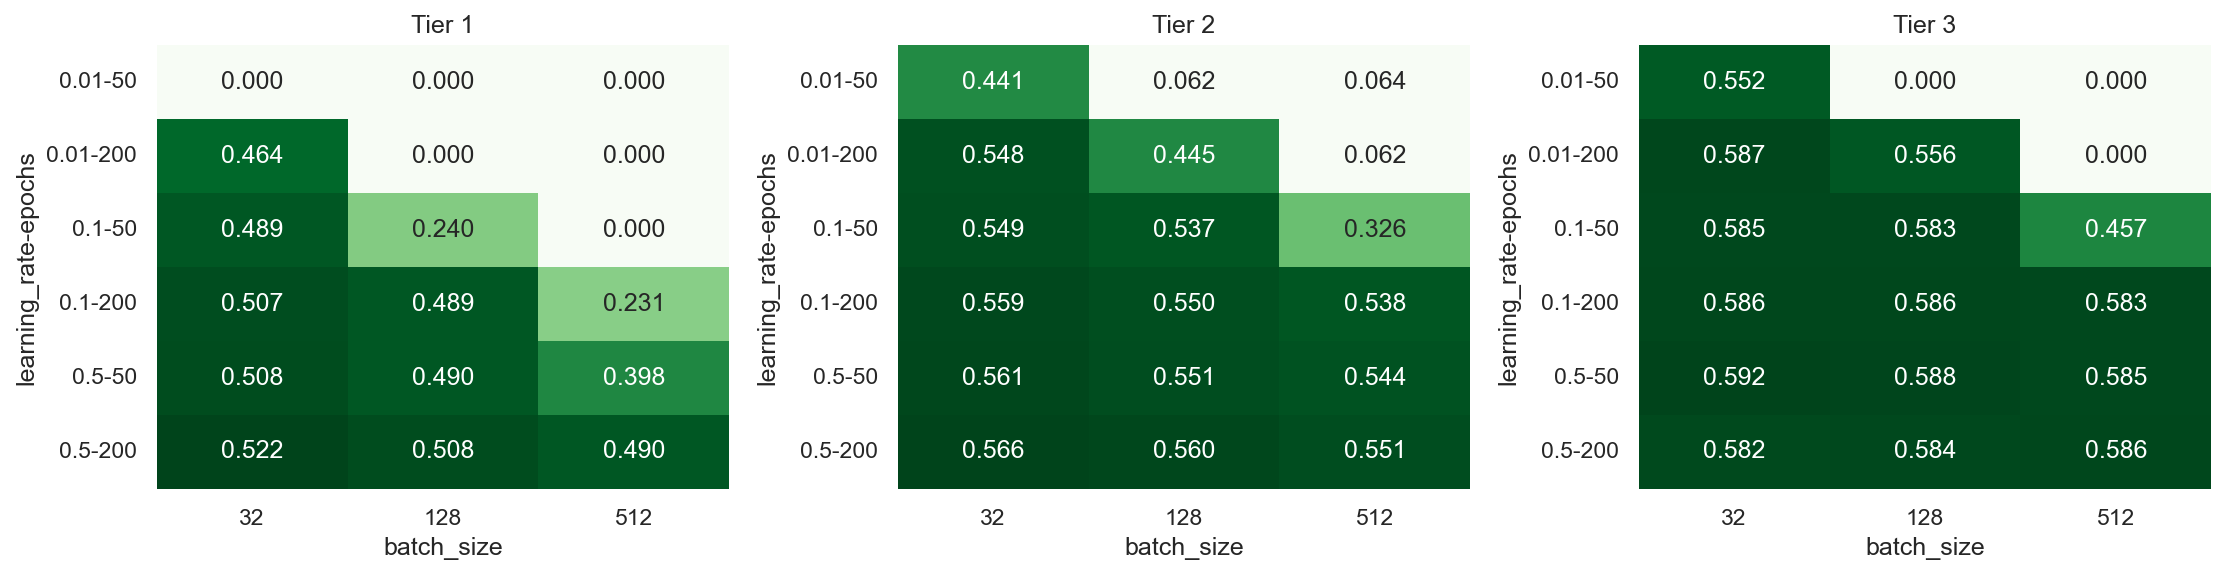
\includegraphics[width=0.8\textwidth]{grid_f_measure.png}
\caption{LR: mean 5-fold CV F-measure of all 18 settings per tier (rows: $\eta$--epochs; columns: batch size).}\label{fig:grid}
\end{figure*}

\subsection{RQ1: Performance Across Tiers}
\textbf{Effect of tiers.} Both models improve with more information (Table~\ref{tab:rq1}). Billing data (Tier~1$\to$2) is the cheapest gain for $k$-NN (F $+0.093$, ROC-AUC $+0.034$) but small for LR (F $+0.027$). Demographics and services (Tier~2$\to$3) add $+0.043$ ($k$-NN) and $+0.057$ (LR) F. So Tier~2, without demographic data, gets 93\% ($k$-NN) to 91\% (LR) of the Tier~3 F-measure.

\textbf{LR vs.\ $k$-NN.} LR has the higher PR-AUC in all three tiers. ROC-AUC is mixed: LR leads by under 0.005 in Tiers~1 and~3, $k$-NN in Tier~2 (0.815 vs.\ 0.807). On F-measure LR wins clearly only in Tier~1 ($+0.051$); $k$-NN wins Tier~2 ($+0.016$) and the Tier~3 gap is only 0.002. Fold standard deviations are 0.02--0.04, so gaps below about 0.02 are within noise.

\textbf{Possible explanations} (plausible, not tested). \emph{Tier~1:} tenure is the only numeric attribute, so many customers are equally far apart and $k$-NN's vote is coarse; LR learns a smooth score instead (negative weights for tenure, one-year contract and dependents). \emph{Tier~2:} Total Charges is roughly tenure $\times$ Monthly Charges; a straight-line score cannot form this product, but similar customers share it, which may favour $k$-NN. \emph{Tier~3:} most of the 40 inputs are 0/1 indicators that each add equally to the distance, so the few that matter get diluted for $k$-NN; LR weights each one separately. We do not read LR weights as causes (contract dummies overlap with the bias).

\begin{table}[t]
\caption{RQ2: mean 5-fold CV F-measure across hyperparameters (development set only).}\label{tab:rq2}
\small\setlength{\tabcolsep}{1.8pt}
\begin{tabular}{@{}llccc@{}}
\toprule
 & & Tier 1 & Tier 2 & Tier 3\\
\midrule
$k$-NN & $k=1$ & 0.477 & 0.524 & 0.497\\
 & odd $k\in[5,19]$ & 0.468--0.507 & 0.546--0.563 & 0.560--0.605\\
 & even $k\in[6,20]$ & 0.430--0.473 & 0.492--0.538 & 0.510--0.597\\
\midrule
LR & all 18 settings & 0.000--0.522 & 0.062--0.566 & 0.000--0.592\\
 & $\eta=0.5$ only & 0.398--0.522 & 0.544--0.566 & 0.582--0.592\\
 & settings with $F{=}0$ & 6 & 0 & 3\\
 & CV ROC-AUC & 0.739--0.807 & 0.783--0.821 & 0.812--0.846\\
\bottomrule
\end{tabular}
\end{table}

\subsection{RQ2: Hyperparameter Sensitivity}
\textbf{$k$-NN} is stable once $k\ge5$ (Table~\ref{tab:rq2}): among odd $k$ the CV F-measure varies by at most 0.045 in any tier, and the best $k$ (15, 13, 19) is fairly large, so more neighbours help. $k=1$ overfits (it copies one neighbour) and is 0.03--0.11 below the best. Even $k$ is always worse than its odd neighbours: an even vote can tie, we predict churn only for a strict majority, so ties become ``no churn'' and recall drops.

\textbf{LR} is much more sensitive (Figure~\ref{fig:grid}). In 9 of the 54 tier-setting pairs it never predicts churn ($F=0$). All are under-trained: a small step size ($\eta=0.01$), or $\eta=0.1$ with a large batch ($|B|=512$), i.e.\ few weight updates. The absolute-error gradient $(1-2y)\hat y(1-\hat y)$ is at most 0.25 and, as non-churners are the majority, early updates mostly push scores down, so a model stopped early scores everyone below 0.5. This is a threshold effect, not missing signal: even at $F=0$ the CV ROC-AUC is at least 0.74, so it already \emph{ranks} customers well. With $\eta=0.5$ the spread shrinks to 0.01--0.12, and every selected setting uses $\eta=0.5$ and $|B|=32$, the edge of our grid. So LR's F-measure depends more on training budget than on features; a grid beyond $\eta=0.5$ is worth trying.

\section{Conclusion}
On this split, administrative and billing data (Tier~2) retain over 90\% of Tier~3 F-measure, with a further gain from demographics and services. Neither model dominates: LR leads on PR-AUC, while $k$-NN is less sensitive to tuning. Restricting features is data minimization, not a privacy guarantee. Results come from a fictional IBM sample and one test split, so they may not generalise to real customers or other splits.

\textbf{Team contributions.} The report sections were divided equally. Abhishek: Abstract and Sections 1, 3, 4 (Introduction, Dataset, Baselines). Dev: Sections 5, 6.2, 7 (Evaluation Strategy, RQ2, Conclusion). Ravi: Sections 2, 6.1 (Research Questions, RQ1).

\textbf{AI use (Category D).} Claude (Anthropic) helped draft this report; OpenAI Codex helped check and edit it against \texttt{output/}. The team remains responsible for the submission.

\bibliographystyle{ACM-Reference-Format}
\bibliography{bibliography}

\end{document}
